
\documentclass{article}
\usepackage{graphicx}
\title{Queries}
\begin{document}

\section{Introduction}
A literature review of C37.118.1-2011 standard  was conducted to find the list of tests to be performed on the PMU setup using mini FSS. But after studying standards, I have a few doubts about its implementation using FSS. These are the tests given in the standard:
\begin{enumerate}
\item Steady-state compliance
	\begin{enumerate}
	\item Steady-state synchrophasor measurement requirements
	\item Steady-state frequency and ROCOF measurement requirements
	\end{enumerate}
\item Dynamic compliance
	\begin{enumerate}
	\item Synchrophasor measurement bandwidth requirements using modulated test signals
	\item Ramp of system frequency
	\item Step changes in phase and magnitude
	\end{enumerate}
\end{enumerate} 
\section{Query -1}
So with the above premise I have a query with \textit{step change test}. Here PMU reporting time will be much longer than the step function time, step function is given at variable steps over period starting from the 1st reporting instance till the next reporting instance in fixed step. From this input the \textit{step response curve} is constructed.

This is made possible in principal (as per the standard) by providing time synchronized test input, viz sampling is time synched (by default) and so is the step function so that the step function can be moved over the given time frame each time. A figure is given below illustrating the point
\begin{figure}[h]
\centering
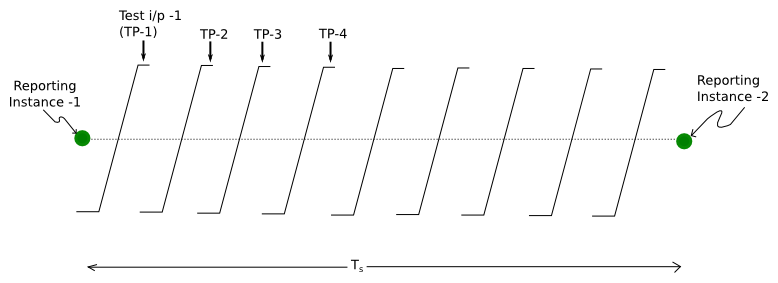
\includegraphics[width=\textwidth]{step_explanation.png}
\caption{test method as per the standard}
\end{figure}

So, my concern is that in our FSS, do we have eithernet connectivity for time synchronization or event triggered signal output using which we can accurately \textit{time } the test signal. As per my conversation with Ajinkya, we dont have such time base or event driven output.

\section{Query-2}

I am bit unclear about objective of our this experiment. So I wanted to ask that are we trying to see the "viability" of FSS as a HIL testing device for PMU and PMU standards? or are we testing our OMAP L-137 based PMU's confirmation with the standards. 
I was bit concerned because the latter would have made sense only if we had CDAC based PMU and not what I am developing as my hardware design is bit primitive yet.

It would be great if you could throw some light on what you were expecting out of this FSS-PMU interfacing experiment with the present status without the C-DAC PMU. 


\end{document}